\subsection{Rotina de Comunicação}
\label{subsec:rotina_comunicacao}
% TODO:
% IDEIA: ILUSTRAR A INTERAÇÃO ENTRE A ROTINA PRINCIPAL E A INTERRUPÇÃO
A rotina de comunicação opera em um \emph{loop} infinito no núcleo principal do microcontrolador e é responsável por tratar os telecomandos recebidos pelo \textit{Bluetooth}. Ao ser identificado um recebimento de mensagem pelo sinal de interrupção da comunicação \textit{Bluetooth} é acionada a função de tratamento de interrupção correspondente que possui como única função encaminhar as mensagens válidas (verificar cabeçalho) para a rotina principal de comunicação. Isso é feito para evitar sobrecarregar a interrupção (podendo atrapalhar as interrupções dos \emph{Encoders} devido à alta prioridade da interrupção). A Figura \ref{fig:ilustracao_rotina_comunicacao} ilustra as etapas da rotina de comunicação.\\

\begin{figure}[H]
    \centering
    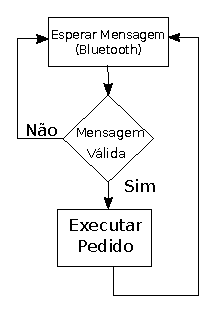
\includegraphics[width=0.3\textwidth]{figuras/ilustracoes/ilustracao_rotina_de_comunicacao.eps}
    \caption{Fluxo grama simplificado da rotina de comunicação.}
    \label{fig:ilustracao_rotina_comunicacao}
\end{figure}

Na rotina principal a mensagem é interpretada e caso ela seja identificada como um telecomando válido, será executada a devida resposta, conforme apresentado mais adiante.

O protocolo implementado foi pensado para conter até três campos básicos, o \textbf{\textit{Header}} com 4 bits (servindo de preâmbulo), para ajudar a sincronizar os pacotes, o identificador de comando \textbf{\textit{CMD}} também com 4 bits, possibilitando assim até 16 comandos distintos e por fim, o campo de argumentos com tamanho variável, (ver Figura \ref{fig:frame_generico}). Foram implementados 7 comandos.

\begin{figure}[H]
    \centering
    \includegraphics[width=0.6\textwidth]{figuras/ilustracoes/ilustracao_frame_generico.eps}
    \caption{Estrutura básica usada na comunicação.}
    \label{fig:frame_generico}
\end{figure}

% Please add the following required packages to your document preamble:
% \usepackage[table,xcdraw]{xcolor}
% If you use beamer only pass "xcolor=table" option, i.e. \documentclass[xcolor=table]{beamer}
\begin{table}[H]
\centering
\begin{tabular}{c|r}
\hline
\rowcolor[HTML]{C0C0C0} 
\multicolumn{1}{|c|}{\cellcolor[HTML]{C0C0C0}DEFINIÇÕES} & \multicolumn{1}{r|}{\cellcolor[HTML]{C0C0C0}VALOR(HEX)} \\ \hline
HEAD & A0 \\
\rowcolor[HTML]{EFEFEF} 
CMD\_REQ\_CAL & 00 \\
CMD\_REQ\_OMEGA & 03 \\
\rowcolor[HTML]{EFEFEF} 
CMD\_CALIBRATION & 04 \\
CMD\_IDENTIFY & 05 \\
\rowcolor[HTML]{EFEFEF} 
CMD\_SET\_POINT & 0A \\
CMD\_CONTROL\_SIGNAL & 0B \\
\rowcolor[HTML]{EFEFEF} 
CMD\_PING & 0F
\end{tabular}
\caption{Definições utilizadas.}
\label{tab:my-table}
\end{table}

A Tabela \ref{tab:defines} apresenta as definições/nomenclaturas utilizadas nas descrições a seguir.

\textbf{Comandos}
\begin{itemize}
    \item \textbf{CMD\_REQ\_CAL}:\\
        \textit{host} envia, para solicitar os dados provenientes da calibração do controlador \textit{Feedforward}. O escravo (robô) envia 4 \emph{Floats}, referente aos coeficientes do controlador.
    \item \textbf{CMD\_REQ\_OMEGA}:\\
        \textit{host} envia, para solicitar as velocidades atuais de ambos os motores, em $rad/s$. O escravo responde com dois \emph{Floats}, referentes aos valores medidos das velocidades correspondentes.
    \item \textbf{CMD\_CALIBRATION}:\\
        \textit{host} envia, para fazer com que o robô inicie sua rotina de calibração do controlador.
    \item \textbf{CMD\_IDENTIFY}:\\
        \textit{host} envia, fazendo com que o robô inicie sua rotina de identificação (rotina que armazena as velocidades durante um certo período de tempo e envia para o \emph{host}, útil para testes). O \textit{host} deve enviar uma mensagem conforme ilustrado na Figura \ref{fig:comando_identify}.\\
        
        \begin{figure}[H]
            \centering
            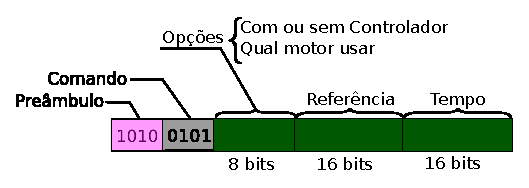
\includegraphics[width=\textwidth]{figuras/ilustracoes/ilustracao_comando_coleta_de_dados.eps}
            \caption{Telecomando para coleta de dados.}
            \label{fig:comando_identify}
        \end{figure}
        
        % % Please add the following required packages to your document preamble:
% \usepackage{graphicx}
% \usepackage[table,xcdraw]{xcolor}
% If you use beamer only pass "xcolor=table" option, i.e. \documentclass[xcolor=table]{beamer}
\begin{table}[H]
\centering
\resizebox{\textwidth}{!}{%
\begin{tabular}{|
>{\columncolor[HTML]{C0C0C0}}l |
>{\columncolor[HTML]{C0C0C0}}l |l|l|l|}
\hline
HEAD & CMD\_IDENTIFY & OPTIONS & SETPOINT & STEPTIME \\ \hline
\end{tabular}%
}
\end{table}
        
        Sendo o campos de opções de 1 byte, contendo a informação de qual motor será feita a identificação e se deve ser usado o controlador.
        
        Ao concluir a rotina de identificação, o robô responde enviando o vetor de velocidades medidas, durante a rotina, para o \textit{host}, que deve estar aguardando recebê-las.
        
        
    \item \textbf{CMD\_SET\_POINT}:\\
        
        \begin{figure}[H]
            \centering
            \includegraphics[width=\textwidth]{figuras/ilustracoes/ilustracao_comando_omega_ref.eps}
            \caption{Telecomando de velocidades de referências.}
            \label{fig:comando_referencia}
        \end{figure}
        
        % % Please add the following required packages to your document preamble:
% \usepackage{graphicx}
% \usepackage[table,xcdraw]{xcolor}
% If you use beamer only pass "xcolor=table" option, i.e. \documentclass[xcolor=table]{beamer}
\begin{table}[H]
\centering
\resizebox{\textwidth}{!}{%
\begin{tabular}{|
>{\columncolor[HTML]{C0C0C0}}c |
>{\columncolor[HTML]{C0C0C0}}c |c|c|c|c|l|l|l|}
\hline
HEAD & CMD\_SET\_POINT & SENSE\_L & OMEGA\_L & SENSE\_R & \multicolumn{4}{c|}{OMEGA\_R} \\ \hline
\end{tabular}%
}

\end{table}
        
        Neste os campos de sentido (conforme Figura \ref{fig:comando_referencia}), como o próprio nome sugere, indicam o sentido de rotação do motor, 0 para trás e 1 para rodar para frente (convertidos em sinal das velocidades de referência) portando só ocupam 1 bit, já os campos referentes às velocidades desejados ocupam 15 bits, sendo assim é possível enviar referências com uma precisão de $1/2^{15}$, já que as referências serão enviadas inteiras  (0 - $2^{15}$) e mapeadas de $-1$ a $1$, indicando uma porcentagem da referência da velocidade máxima do robô. Ou seja os campos referentes às referências contêm valores proporcionais à velocidade máxima do robô.
        
    \item \textbf{CMD\_CONTROL\_SIGNAL}:\\
        
        \begin{figure}[H]
            \centering
            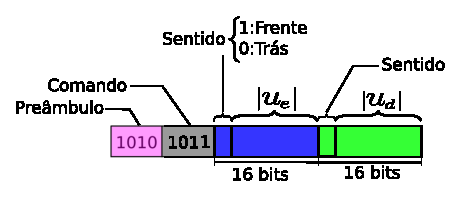
\includegraphics[width=\textwidth]{figuras/ilustracoes/ilustracao_comando_sinal_de_controle.eps}
            \caption{Telecomando de sinal de controle.}
            \label{fig:comando_sinal_de_controle}
        \end{figure}
        
        O comando difere apenas no campo de comando do telecomando anterior. O restante da estrutura é exatamente igual, pois a principal diferença ocorre no microcontrolador. Em vez dos campos referentes às velocidades de referência, neste comando o robô irá interpretar esses campos como contendo sinais de controle (após convertê-los para \emph{float} de $-1$ a $1$).
        
    \item \textbf{CMD\_PING}:\\
        Neste comando o \textit{host} pode enviar qualquer mensagem no campo de argumentos, pois o robô irá apenas responder com a mesma mensagem. Este comando é útil para testar conexão e testar a latência da conexão.
    
\end{itemize}